\chapter{National Governments' Administration on Intergovernmental Transfer}

\section{Literature on Game Theory Modeling of Bargaining Process}
In the United States, approximately \$700 billion, which constitutes almost 20\% of the federal revenues, is annually disbursed across various state and local government grant programs. As a result, the mechanism by which intergovernmental transfers are distributed has long been a captivating subject in public finance.

The distribution of grants in democratic countries is considered a bargaining game among decision-making groups such as committees, congress, or houses, depending on which group is the decisive institution.  Four assumptions are crucial in simulating the grants distribution bargaining using bargaining models: recognition rule, voting rule, amendment rule, and money-distribution rule. The recognition rule determines how to select an agenda setter to make the initial proposal, with most literature assuming the random recognition rule \cite{kalandrakis2004three,anesi2015bargaining,diermeier2011legislative,rosenstiel2021congressional}, which means $n$ members among the decision making institution have equal probabilities to be chosen to make the initial proposal. The voting rule establishes the standard for passing the proposal, with the majority rule and unanimous voting rule being common. The amendment rule places constraints on making amendments, ranging from the closed rule, which allows no amendments, to the open rule, which allows any and all (germane) amendments.Finally, the grants-type rule determines how grants could be manipulated by decision-making institutions, with some scholars assuming direct decisions on the number of receivers, referred to as "earmarks" or "pork barrel" spending model. The mechanism of intergovernmental transfer distribution, which accounts for nearly 20 percent of overall federal revenues, is a compelling topic in the public finance area, particularly in democratic countries like the United States.

Baron and Ferejohn's work \cite{baron1989bargaining} laid the foundation for subsequent analyses of bargaining models. They made several important assumptions, such as random recognition, majority voting rule, and earmarks rule. Their work, as well as the generalization by Banks and Duggan \cite{banks2006general}, demonstrates that legislators with agenda-setting power tend to receive a disproportionate share of funding. In addition, the equilibrium is characterized by funds flowing only to legislators in the winning coalition, with no funds allocated to those outside of it. Furthermore, they found that when proposals are brought up under a closed rule, the winning coalition is minimized, leading to the maximization of benefits for the members of the winning coalition.

Although Baron and Ferejohn's work \cite{baron1989bargaining} is pioneering in the field of grants distribution, the heavy reliance on the "earmarks" assumption limits its explanatory power in the actual political environment. Martin \cite{martin2018dividing} addresses this issue by modifying the assumptions of the model. Specifically, he restricts the power of decision-making members to only determine the factors in the formula rather than the specific numbers. This modification is a significant step towards reflecting the realities of political and administrative life. Martin's model generates different conclusions compared to Baron and Ferejohn's work. In contrast to the latter, Martin predicts oversized winning coalitions and the emergence of persistent winning blocs. Additionally, he demonstrates that when bargaining over a low-dimensional formula, legislators have limited ability to target funds to specific districts, a prediction supported by empirical evidence. For instance, Martin analyzed existing formula grants and found that 95\% of the formula have less than 5 variables, which means members have limited bargaining dimensions. As a result, jurisdictions with similar features can be free-riders, even if they are not part of the winning coalition. Martin predicts positive distribution outside the winning coalition as a consequence.

\section{Some Empirical Evidence for the Grants Distribution}

Apart from the introductory remarks on intergovernmental transfers in Chapter 1, one of the primary challenges with their distribution is the political environment in which it occurs. The allocation of intergovernmental transfers is often susceptible to the influence of individual political agendas that may undermine the intended structure of the distribution procedures. This challenge has been addressed through classic game theory analyses of Congress. Given the significant role of intergovernmental transfers in the US federal system, the influence of politics on their allocation can be prohibitively expensive. Several anecdotal examples illustrate this, such as Robert Carlyle Byrd's efforts to direct federal spending to his home state, West Virginia, over two decades. One example of Robert Byrd's influence is seen in the creation of a new formula for distributing a trust fund surplus proposed by him during the 1992-1997 authorization negotiation. This new formula primarily benefited states such as West Virginia with high state gasoline tax rates and low per capita income.

Markusen, Saxenian and Weiss's \cite{markusen1981benefits}conducted a descriptive study to analyze three distinct swings in the distribution of federal grants to cities during the 1960s and 1970s. They found that federal grants increased substantially during this period, with northeastern and midwestern cities benefiting the most from 1965-1972, southern and western cities benefiting the most from 1972-1975, and a slight swing back in favor of the first group from 1975-1978. These swings can be partially explained by the political background, as noted in their article. Stegarescu \cite{stegarescu2006decentralised} explains that the degree of IGT decentralization is a result of population, unemployment, trade-openness, presidential regimes and electoral systems based on the test result of the panel data of 17 nations. Kasdin \cite{kasdin2016decision} conducted an empirical test and found that the complexity of state or local government networks influences the amount of federal transfer and federal control. Higher-level governments tend to relinquish control when the lower governmental network is highly complicated, but the amount of transfer is negatively related to complexity. The complexity can be a barrier that hinders politicians from claiming political credit, and thus, they are less motivated to secure fiscal revenue for their jurisdiction. Larcinese, Rizzo, Testa \cite{larcinese2006allocating} tested the impact of the president on the amount of federal transfer to state government and found that states that heavily supported the incumbent president in past presidential elections tend to receive more funds. Wallis \cite{wallis1987employment} also emphasizes the political effect on the amount of intergovernmental transfer. He claims that states with the high volatility of presidential vote receive significantly more federal support based on his study on the longitudinal data of all states in the U.S. Markusen, Saxenian and Weiss \cite{markusen1981benefits} defined the supply side and demand side when investigating the mechanism of the IGTs decision-making process, even though they don’t point out the specific factors, they emphasize that the IGT is the result of the political, economic and social characteristics of both demand and supply side.

The existing literature suggests that political factors, including potentially biased factors, can significantly impact the distribution of intergovernmental transfers. Based on the aforementioned studies, it can be inferred that the determinants of intergovernmental transfers are not limited to legislative decision-making institutions, but also include administrative branches. Furthermore, the political stance of local jurisdictions appears to play a notable role in intergovernmental distribution.

\section{An Empirical Investigation on IGT Distribution Mechanism}
Combined with Martin's \cite{martin2018dividing} conclusion introduced in section 2.2.1 and all the literature implying the political impact mentioned above, I design and conduct an longitudinal empirical test to statistically investigate the intergovernmental transfer mechanism. Specifically, I try to solve two questions in this empirical design, for one, following Martin's inference, how much extent does states share similar characteristics so the IGT benefits goes outside of the winning coalition. Another questions I wander is, following Markusen, Saxenian and Weiss's framework, if we got the social and economic characteristics control, how much can political factors affect the IGT. The reason I focus on the political factors is that, contradictory to what we discussed in section 2.1, the political factor seems unrelated to efficiency, thus may cause more distortion and waste of resources. Besides, examination on political factors could be important because of the sharp rise in hostility between democratic and republican parties. The potential effects of political party control may impact the IGT grants distribution significantly.

\subsection{Sample and Characteristic Selection}
I focus on the direct IGT from federal government to state governments in America. To incorporate the political impact into the data framework, I did a stratified sampling to collect states sample from traditional republican states, traditional democratic states and swing states.
The state grouping method are based on two criterion, the historical presidential election result and the winning rate following Beachler,Donald,Bergbower,Matthew etc.'s work \cite{beachler2015presidential}. The democratic states and republican states are those chose same party in the president election since 1984 with wining rate over 58\%. The swing states are those have chosen president from two parties and the winning rates are less than 58\%.

The states collected into my sample can be listed as Table \ref*{Table 2.3}

% Table generated by Excel2LaTeX from sheet 'Sheet1'
\begin{table}[H]
    \centering
    \caption{States Sample and Grouping}
    \begin{tabular}{p{7.57em}cc}
        \toprule
        States         & \multicolumn{1}{p{7.93em}}{Group}                    & \multicolumn{1}{p{6.855em}}{Code} \\
        \midrule
        Wyoming        & \multicolumn{1}{c}{\multirow{5}[2]{*}{Red States}}   & \multirow{5}[2]{*}{1}             \\
        Idaho          &                                                      &                                   \\
        Kansas         &                                                      &                                   \\
        Nebraska       &                                                      &                                   \\
        North Dakota   &                                                      &                                   \\
        \midrule
        Maryland       & \multicolumn{1}{c}{\multirow{5}[2]{*}{Blue States}}  & \multirow{5}[2]{*}{2}             \\
        Massachusetts  &                                                      &                                   \\
        Rhode Island   &                                                      &                                   \\
        New York State &                                                      &                                   \\
        Washington     &                                                      &                                   \\
        \midrule
        Pennsylvania   & \multicolumn{1}{c}{\multirow{4}[2]{*}{Swing States}} & \multirow{4}[2]{*}{3}             \\
        Nevada         &                                                      &                                   \\
        Wisconsin      &                                                      &                                   \\
        Ohio           &                                                      &                                   \\
        \bottomrule
    \end{tabular}%
    \label{Table 2.3}%
\end{table}%

The social and economic characteristics that commonly included in the formula when doing the intergovernmental transfer are population, working age population weight, median household income, unemployment rate, road mileage and gdp \cite{dilger2015federal}. I collected all factors mentioned in Dilger's service\cite{dilger2015federal} of the sample states, besides, I also take reference from some major intergovernmental transfer programs such as Medicaid, the Title I-A education program, Temporary Assistance for Needy Families (TANF), Section 8 Housing Choice Vouchers, and the Community Development Block Grant (CDBG) to collect factors comprehensively. I also did proper operation for data regression convenience and better data visualization. The characteristics I collected and source of data can be listed as Table \ref*{Table 2.4}.

\begin{table}[H]
    \centering
    \caption{Social characteristics for Sample States}
    \begin{tabular}{cp{6.43em}p{9.285em}p{5.855em}p{5.355em}}
        \toprule
        \multicolumn{1}{p{4em}}{Variables } & Definition                      & Operation          & Source                              & Time Period                  \\
        \midrule
        gdp                                 & \multicolumn{1}{c}{Real GDP}    & Log transformation & FRED                                & 2000-2019 annually collected \\
        \midrule
        lgp                                 & \multicolumn{1}{c}{Population } & Log transformation & Census of bureau                    & 2000-2019 annually collected \\
        \midrule
        wapw                                & Working age population weight   & No operation       & Census of bureau                    & 2000-2019 annually collected \\
        \midrule
        mhi                                 & State median household income   & Log transformation & Census of bureau                    & 2000-2019 annually collected \\
        \midrule
        ur                                  & unemployment rate               & No operation       & FRED                                & 2000-2019 annually collected \\
        \midrule
        prm                                 & public road mileage             & Log transformation & Bureau of transportation statistics & 2000-2019 annually collected \\
        \bottomrule
    \end{tabular}%
    \label{Table 2.4}%
\end{table}%


\subsection{Principle Components Analysis of Social and Economic Characteristics}
%%principle components analysis
%%%%%%%%%%%%%%%%%%%%%%%%%%%%%%%%%%%%%%%%%%%%%%%%%%%%%%
As mentioned previously, the formula for distributing grants may involve numerous factors. Furthermore, issues of multicollinearity can be intuitively identified within the variables that have been collected. For instance, the weight of the working-age population and the unemployment rate are highly interdependent variables, where higher population levels inevitably correspond to increased utilization of public roads. This observation is further supported by the correlation heatmap, which indicates a certain degree of correlation among the variables.
\begin{figure}[H]
    \centering
    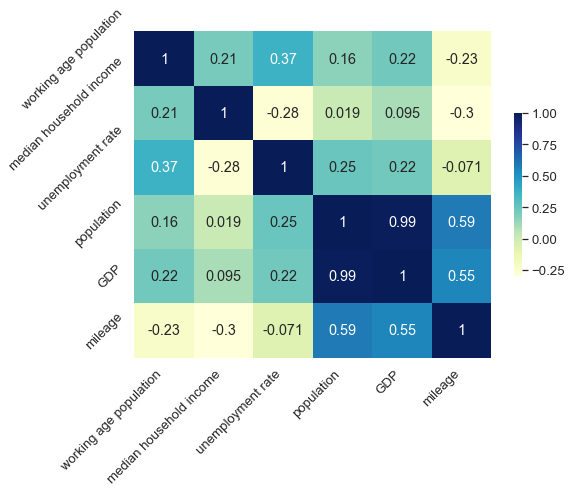
\includegraphics[scale=0.7]{Chapter-3/Figures/heatmap.png}
    \caption[Heatmap of the Social Characteristics]{Heatmap of the Social Characteristics
        \texttt{} }
    \label{heatmap}
\end{figure}

To answer the first question,these two problems are obvious hinder thus it's hard to judge how similar jurisdictions could be in social and economic characteristics directly. So I conduct a primary components analysis to reduce the data dimension and overcome multicollinearity problem to check if the reduced-dimension data are cluster distributed or scattered distributed.

According to the primary components variance analysis result shown in the figure, the first two dimensions express 67\% of the information. The first three dimensions include 87\% of the information.

\begin{figure}[H]
    \centering  %居中
    \subfigure[Histgram]{   %第一张子图
        \begin{minipage}{7cm}
            \centering    %子图居中
            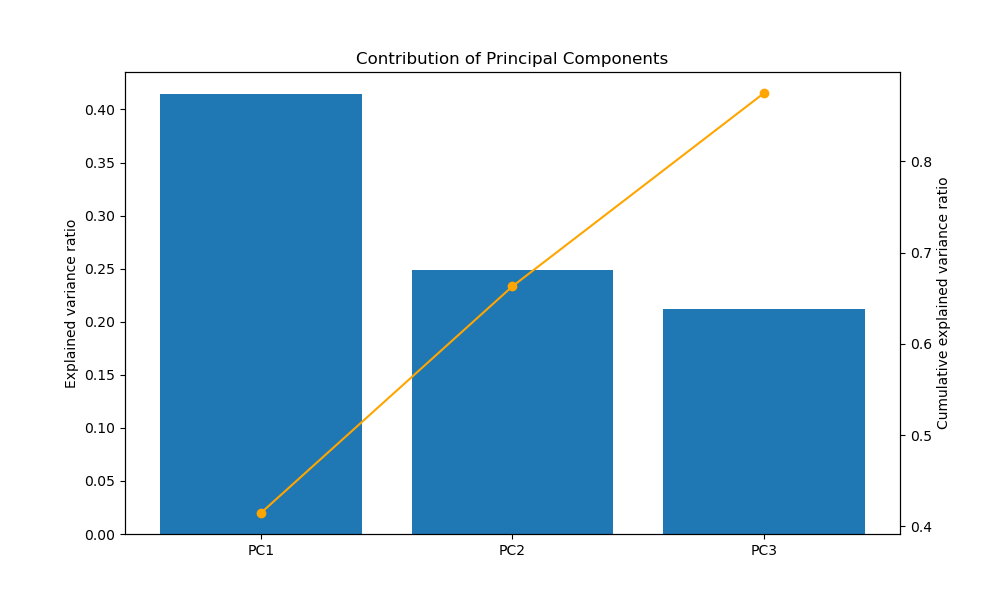
\includegraphics[scale=0.2]{Chapter-3/Figures/contribution.png}  %以pic.jpg的0.5倍大小输出
        \end{minipage}
    }
    \subfigure[Line]{ %第二张子图
        \begin{minipage}{7cm}
            \centering    %子图居中
            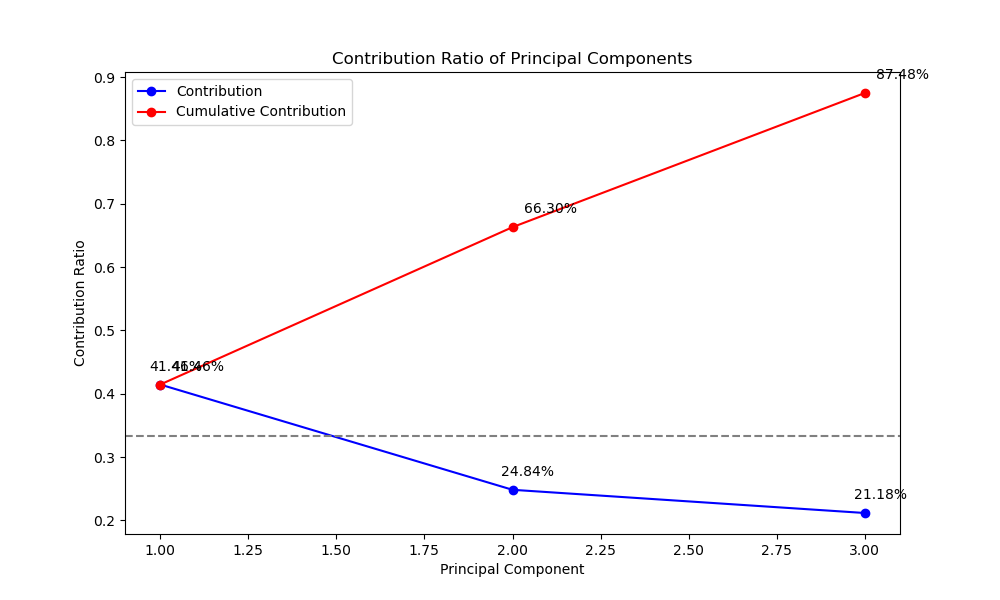
\includegraphics[scale=0.2]{Chapter-3/Figures/contribution2.png}%以pic.jpg的0.5倍大小输出
        \end{minipage}
    }
    \caption[Principle Components Contribution]{Principle Components Contribution}    %大图名称
    \label{principlecomponentcontribution}    %图片引用标记
\end{figure}


Thus I did principle components analysis by compress the data into two and three dimensions separately. By keeping these two and three principle components with most information, comparing the characteristics between jurisdictions became a possible procedure. The scatter plot after data dimension reduction is shown as Figure \ref*{Figure 2.2}

% \begin{figure}[H]
%     \centering
%     \includegraphics[scale=1]{Chapter-2/Figures/pca.png}
%     \caption[Social Characteristics Principle components Analysis]{Social Characteristics Principle Component Analysis
%         \texttt{} }
%     \label{Figure 2.2}
% \end{figure}

\begin{figure}[H]
    \centering  %居中
    \subfigure[2 Principle Components Analysis Scatter]{   %第一张子图
        \begin{minipage}{7cm}
            \centering    %子图居中
            \includegraphics[scale=0.45]{Chapter-3/Figures/pca.png}  %以pic.jpg的0.5倍大小输出
        \end{minipage}
    }
    \subfigure[3 principle Components Analysis Scatter]{ %第二张子图
        \begin{minipage}{7cm}
            \centering    %子图居中
            \includegraphics[scale=0.45]{Chapter-3/Figures/pca_3d.png}%以pic.jpg的0.5倍大小输出
        \end{minipage}
    }
    \caption[Principle Components Analysis Scatter Plot]{Social Characteristics Principle Components Analysis Scatter Plot}    %大图名称
    \label{Figure 2.2}    %图片引用标记
\end{figure}

Though reduced dimensions do not have specific economic meaning, but one clear information shown in Figure \ref*{Figure 2.2} is that a lot of states characteristics are cluster distributed, which means plenty jurisdiction features in my data are quite are quite similar. This implication is a side evidence for Martin's \cite{martin2018dividing} deduction that some jurisdiction with similar features can be a free riders, this also predicts the funds outflow of the winning coalition.

Another potential implication is that, the distribution is obviously hierarchical in terms political parties. Republican states, democratic states and swing states are clearly cluster distributed in their own area. In 2d plot shown in Figure \ref*{Figure 2.2} (a) , Red dots and blue dots distributes on two sides while swing states in the middle. This means any modification on the grants formula that benefits one party is a huge damage to another. This may explain why in the legislative bargaining process, two parties are sharply opposed and swing states are relatively indifferent. What makes Swing states different from the other parties is implied in the 3-D plot shown in Figure \ref*{Figure 2.2} (b), the green dots are not in the same level in the third dimension. This is not counterintuitive, since traditional republican states are highly likely to share similar social characteristics, but this figure may offer a different view on any fiscal collective behavior of the party. When a member in the bargaining process take any behavior, are they doing that due to their political status or arguing benefits for their represented jurisdiction? It seems that any collective political behavior within a party should find a micro-foundation. In other words, when analyze the motivation, one should focus on the motivation of particular member rather than the motivation of a whole group.

\subsection{Political Impact Investigation}
%%political factor regression
%%%%%%%%%%%%%%%%%%%%%%%%%%%%%%%%%%

The goal of this section is to  develope and test a theoretical framework that seeks to further advance the understanding of how the above factor outside of the bargaining institution can affect the spatial distribution of IGT. I still focus on the intergovernmental transfer from federal to state governments. Toward this end, based on the literature implication I collected in section 2.2.1 and 2.2.2, I explore how combination of political party control across legislative and administrative branches affects the distribution of IGT. The factor I'm interested includes whether legislative and administrative branches is unified, whether Democratic or Republican party has different preferences, and whether party control is aligned across the federal and state governments. The distribution of IGT is affected by (1) political party distribution across the federal and state government, and by (2) political party affiliation (i.e., Republican or Democratic party). I also examine how the perceived importance of a state in the federal political process affects the distribution of IGT. In addition, to gain insight into the role of swing state,I also examine the relationship between the IGT and whether a particular state is considered a battle ground state.

\subsubsection{Variable and Data}
The variables I collected can be listed as Table \ref*{Table 2.5}, the data is annually collected from 20000 to 2019, and the source of the data and other detail is attached in Appendix Table\ref*{Table A.1}.

One variable I need to explain here is the dummy variable $c$, which represents the party distribution combination in administrative and legislative branch across federal and state levels.


\begin{table}[htbp]
    \centering
    \caption{Variables and Operation}
    \begin{tabular}{lcp{12.715em}p{6.145em}}
        \toprule
        \multicolumn{2}{p{9.93em}}{Variables }                        & Definition & Operation                                                                                    \\
        \midrule
        \multicolumn{1}{p{4.715em}}{Dependent Variable}               & lg(igt)    & IGT from federal to state i                               & Log                              \\
        \midrule
        \multicolumn{1}{l}{\multirow{2}[4]{*}{Independent Variables}} & c          & Combinations of levels, branches and parties.             & \multirow{2}[4]{*}{No operation} \\
        \cmidrule{2-3}                                                & p          & Dummies to identify i is democratic, republican or swing. & \multicolumn{1}{c}{}             \\
        \midrule
        \multicolumn{1}{l}{\multirow{6}[12]{*}{Control Variables}}    & log(gdp)   & \multicolumn{1}{l}{Real GDP}                              & \multirow{4}[8]{*}{Log }         \\
        \cmidrule{2-3}                                                & log(pl)    & \multicolumn{1}{l}{Population }                           & \multicolumn{1}{c}{}             \\
        \cmidrule{2-3}                                                & wapw       & Working age population weight                             & \multicolumn{1}{c}{}             \\
        \cmidrule{2-3}                                                & mhi        & State median household income                             & \multicolumn{1}{c}{}             \\
        \cmidrule{2-4}                                                & ur         & unemployment rate                                         & No operation                     \\
        \cmidrule{2-4}                                                & prm        & public road mileage                                       & Log                              \\
        \bottomrule
    \end{tabular}%
    \label{Table 2.5}%
\end{table}%

Three aspects decide the type of "$c$", which are the governmental level, branches and different parties. 2 Branches and 2 levels formulate a $2\times2$ Table shown in Table \ref*{Table 2.6}, which are four sectors. For each sector,$ u_1, u_2, s_1, s_2,$ two possible parties may get control, which are the democratic party "$d$" and the republican party "$r$". For example, $c_1 = (u_1 = r, u_ = r, s_1 = r, s_2 = r)$, where ’r’ means republican party and ’d’ means democratic party. Here, I just use abbreviation $(r,r,r,r)$ to express $c_1$, which means combination one. In this research, I use the majority of the House of Representatives to define the partyism of the legislative branch since the House plays a leading role in the budget making process. The partyism of the administrative branch is decided by the partyism of the administrative leader, which could be the president or governor. There are 16 types of combination, which are:
$$(r, r, r, r), (r, r, r, d), (r, r, d, r), (r, r, d, d), (r, d, r, r), (r, d, r, d), (r, d, d, r), (r, d, d, d)$$\\$$(d, r, r, r), (d, r, r, d), (d, r, d, r), (d, r, d, d), (d, d, r, r), (d, d, r, d), (d, d, d, r), (d, d, d, d) $$

I use $c_1, c_2, . . . c_{16}$ to express these 16 different combinations. In the regression,
only fifteen combinations are saved, the first combination $c_1 = (r, r, r, r)$ is omitted in regression to avoid the multicollinear problem and $c_1$ acts as a benchmark.

% Table generated by Excel2LaTeX from sheet 'Sheet1'
\begin{table}[H]
    \centering
    \caption{Branches and Levels Combination}
    \begin{tabular}{cp{7.145em}p{8.43em}p{6.145em}}
        \toprule
        \multicolumn{2}{c}{\multirow{2}[4]{*}{}}       & \multicolumn{2}{p{14.575em}}{Branches}                 \\
        \cmidrule{3-4}    \multicolumn{2}{c}{}         & administrative                         & house         \\
        \midrule
        \multicolumn{1}{c}{\multirow{2}[4]{*}{Levels}} & federal                                & $u_1$ & $u_2$ \\
        \cmidrule{2-4}                                 & state level                            & $s_1$ & $s_2$ \\
        \bottomrule
    \end{tabular}%
    \label{Table 2.6}%
\end{table}%

As for dummy variable $p$, I collected the longitudinal data of three different types of states based on whether the states are traditional democratic states, republic states, or swing states, Fifteen states are divided into 3 groups. The first group is the traditional republican states group, or what are called "red wall states", and we code $p = 1$ for the first group. Second group is traditional democratic state group, also known as “blue wall states”, and we define $p = 2$ for second group. The third group is the swing state group, also known as the "battle ground states", $p = 3$ for the third group. The sample states in this research is same as the sample in principle components analysis collected in Table \ref*{Table 2.3}.

I selected some variables and generate some relationship scatter plots to get a intuitive description about the relationship. The figure is shown in Figure \ref*{Figure 2.3}. I hide the legend of different party. One thing that should be noticed is that, except for the lower left subfigure, which shows the relationship between relationship and igt, shows a clear linear trend, other figures show obvious hierarchical distribution. The linear relationship between population and intergovernmental transfer amount is not surprising, but the hierarchical plot is kind of intriguing, hold x axis constant, we still get different igt amounts. Even for the relationship between the partisan of states and IGT amounts, especially for those democratic states, the points falls on both upper and lower sides. The hierarchical distribution implies that the social and economic characteristics cannot fully explains the IGT distribution, and the rest of the black box may potentially be explained by political impact and the influence out of the legislative branch.

\begin{figure}[H]
    \centering
    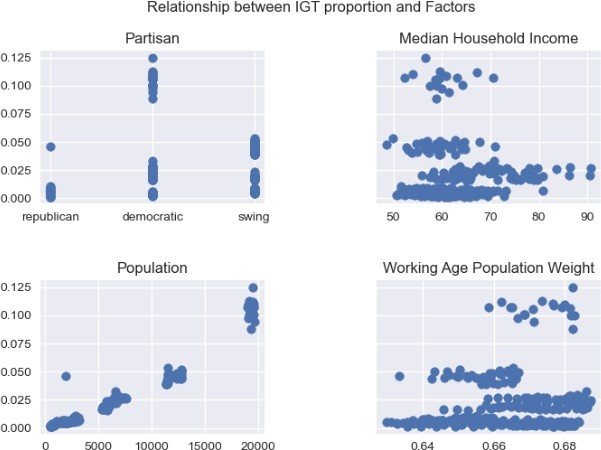
\includegraphics[scale=1]{Chapter-3/Figures/IGT and factors.jpg}
    \caption[IGT and Factors Scatter Plot]{Factor and IGT Scatter Plot
        \texttt{} }
    \label{Figure 2.3}
\end{figure}

\subsubsection{Model Setting}
Though I did a relatively comprehensive literature investigation in grants distribution formula issue, and the sample data includes the most important concerns in intergovernmental transfer distribution, it still possible that some variables may be omitted from the equation, especially given this is a longitudinal data with 19 years time span. So one crutial problem for this investigation is how to deal with the potential omitted variable issue and avoid the following heteroscedasticity and endogenity problem. To make sure I can get an unbiased estimate, I adopt two factor fixed effect model in the regression. In the following researech, I display 3 regression models. The benchmark model is OLS regression. Besides, since the fiscal behavior happens on state level, which is a relatively big and stable jurisdiction, it's totally possible some factors are time-invariant. So, the second model in my display is fixed model with time variable fixed. Though, state is a relatively stable jurisdiction, the time span is relatively long, thus some omitted variables could be time-variant as well. To get all these omitted variables controlled as much as possible, the third model I adopt is two factor fixed effect model, with both time factor and individual effect controlled.

The equation for OLS regression can be displayed as follow.
\begin{equation}
    \begin{split}
        log(igt_{i,t}) & = \alpha + \beta_1 c_{i,t} + \beta_2 p_{i,t} + \beta_3 log(gdp) + \beta_4 log(pl) + \beta_5 log(mhi_{i,t}) \\
        & + \beta_6 wapw_{i,t} + \beta_7 ur_{i,t} +\beta_8 log(prm_{i,t}) + \epsilon_{i,t}
    \end{split}
\end{equation}
$For\ t = 1, 2, 3...T\ and\ i = 1, 2, 3...N $

The second model, which is the fixed effect model with time effect fixed is:
\begin{equation}
    \begin{split}
        log(igt_{i,t}) & = \alpha_i + \beta_1 c_{i,t} + \beta_2 p_{i,t} + \beta_3 log(gdp) + \beta_4 log(pl) + \beta_5 log(mhi_{i,t}) \\
        &+ \beta_6 wapw_{i,t} + \beta_7 ur_{i,t} +\beta_8 log(prm_{i,t}) + \epsilon_{i,t}
    \end{split}
\end{equation}
$For\ t = 1, 2, 3...T\ and\ i = 1, 2, 3...N $

Finally, the third model, which is two factor fixed effect model with time effect and individual effect controlled is:
\begin{equation}
    \begin{split}
        log(igt_{i,t}) & = \alpha_i + \theta_t + \beta_1 c_{i,t} + \beta_2 p_{i,t} + \beta_3 log(gdp) + \beta_4 log(pl) + \beta_5 log(mhi_{i,t}) \\
        &+ \beta_6 wapw_{i,t} + \beta_7 ur_{i,t} +\beta_8 log(prm_{i,t}) + \epsilon_{i,t}
    \end{split}
\end{equation}

$For\ t = 1, 2, 3...T\ and\ i = 1, 2, 3...N $

There are four hypothesis in this investigation, which can be listed as follow.

\textbf{Hypothesis 1–The unified Government Hypothesis}

Unified government means the administrative branch and legislative branch on federal level coming from same party. Unified government is likely to spend a higher overall spending scale since the financial powers are less limited.

\textbf{Hypothesis 2–Party Specific Hypothesis}

Democratic and republican parties have different preferences on the IGT scale. The preference on IGT of different parties is fuzzy here, since two possible inference may be reasonable here. In terms of the scale of government, the democratic party prefers a big government, which would lead to a higher-scale IGT, and the republican party holds the opposite idea. In terms of the administrative structure, democratic government tends to establish a centralized government, whereas republican government prefers a decentralized structure. In this way, we can get a opposite conclusion

\textbf{Hypothesis 3–Alignment Hypothesis}

The allocation of the IGT are affected by the political ideology. The federal government is likely to allocate more IGT to states that are controlled by same party.

\textbf{Hypothesis 4–Battle Ground States Hypothesis}

The competition level between two parties in state would affect the IGT received by that state government. The federal government is motivated to get elected or reelected; thus, the federal government is willing to put resources and supply more public goods to states that matter a lot for their election to get political credits.

The regression results can be summarized as Table \ref*{Table 2.7}
% Table generated by Excel2LaTeX from sheet 'Sheet3'
\begin{table}[H]
    \centering
    \caption{Regression Results Display}
    \begin{tabular}{cccc}
        \toprule
                                        & \multicolumn{1}{p{7.645em}}{Model-1}  & \multicolumn{1}{p{7.5em}}{Model-2}  & \multicolumn{1}{p{8.07em}}{Model-3}  \\
                                        & \multicolumn{1}{p{7.645em}}{Log(igt)} & \multicolumn{1}{p{7.5em}}{Log(igt)} & \multicolumn{1}{p{8.07em}}{Log(igt)} \\
        \midrule
        \multicolumn{1}{p{6.93em}}{c2}  & -0.0161                               & -0.0534                             & -0.0954                              \\
                                        & -0.43                                 & -1.99                               & -1.83                                \\
        \multicolumn{1}{p{6.93em}}{c3}  & -0.0467                               & -0.0352                             & 0.0282                               \\
                                        & -1.4                                  & -1.4                                & -1.09                                \\
        \multicolumn{1}{p{6.93em}}{c4}  & 0.00886                               & -0.0751                             & -0.101                               \\
                                        & -0.19                                 & -2.21                               & -2.67                                \\
        \multicolumn{1}{p{6.93em}}{c5}  & -0.127                                & -0.122                              & 0.-0768                              \\
                                        & -3.31                                 & -3.12                               & -2.87                                \\
        \multicolumn{1}{p{6.93em}}{c6}  & 0.0792                                & 0.0203                              & 0.0351                               \\
                                        & -1.33                                 & -0.47                               & -0.73                                \\
        \multicolumn{1}{p{6.93em}}{c7}  & -0.0125                               & 0.00947                             & 0.0149                               \\
                                        & -0.32                                 & -0.27                               & -0.51                                \\
        \multicolumn{1}{p{6.93em}}{c8}  & 0.0578                                & 0                                   & 0.0767                               \\
                                        & -1.3                                  & 0                                   & -2.15                                \\
        \multicolumn{1}{p{6.93em}}{c9}  & 0.0314                                & 0.0368                              & 0.00131                              \\
                                        & -1.32                                 & -1.21                               & -0.08                                \\
        \multicolumn{1}{p{6.93em}}{c10} & -0.0601                               & -0.0392                             & -0.0318                              \\
                                        & -1.27                                 & -1.2                                & -0.76                                \\
        \multicolumn{1}{p{6.93em}}{c11} & 0.144                                 & 0.127                               & 0.0973                               \\
                                        & -1.6                                  & -1.87                               & -1.5                                 \\
        \multicolumn{1}{p{6.93em}}{c12} & 0.0561                                & 0                                   & 0.0692                               \\
                                        & -1.26                                 & 0                                   & -1.94                                \\
        \multicolumn{1}{p{6.93em}}{c13} & 0.0963                                & 0.078                               & 0.0371                               \\
                                        & -1.96                                 & -1.78                               & -1.07                                \\
        \multicolumn{1}{p{6.93em}}{c14} & 0.0653                                & 0.021                               & -0.00931                             \\
                                        & -0.81                                 & -0.4                                & -0.15                                \\
        \multicolumn{1}{p{6.93em}}{c15} & 0.000495                              & -0.0173                             & 0.00997                              \\
                                        & -0.01                                 & -0.33                               & -0.21                                \\
        \multicolumn{1}{p{6.93em}}{c16} & 0.0466                                & 0                                   & 0.0512                               \\
                                        & 1.94                                  & 0                                   & 2.44                                 \\
        \bottomrule
    \end{tabular}%
    \label{Table 2.7}%
\end{table}%

% Table generated by Excel2LaTeX from sheet 'Sheet3'
\begin{table}[htbp]
    \centering
    \caption{Regression Results Display (follow up)}
    \begin{tabular}{p{6.93em}ccc}
        \toprule
        \multicolumn{1}{c}{}          & \multicolumn{1}{p{7.645em}}{Model-1}  & \multicolumn{1}{p{7.5em}}{Model-2}  & \multicolumn{1}{p{8.07em}}{Model-3}  \\
        \multicolumn{1}{c}{}          & \multicolumn{1}{p{7.645em}}{Log(igt)} & \multicolumn{1}{p{7.5em}}{Log(igt)} & \multicolumn{1}{p{8.07em}}{Log(igt)} \\
        \midrule
        Democratic States             & 0.259                                 & 0.217                               & 0                                    \\
        \multicolumn{1}{c}{}          & -4.88                                 & -5.51                               & 0                                    \\
        Swing States                  & 0.0899                                & 0.0189                              & 0                                    \\
        \multicolumn{1}{c}{}          & -2.7                                  & -1.94                               & 0                                    \\
        Log(population)               & 0.106                                 & 1.087                               & 0.457                                \\
        \multicolumn{1}{c}{}          & -0.92                                 & -10.67                              & -1                                   \\
        working age population weight & -5.362                                & 2.199                               & -4.768                               \\
        \multicolumn{1}{c}{}          & -6.93                                 & -2.72                               & -5.43                                \\
        Log(median household income)  & -0.753                                & -1.407                              & -0.348                               \\
        \multicolumn{1}{c}{}          & -3.51                                 & -8.68                               & -1.26                                \\
        unemployment rate             & 0.0136                                & -0.0151                             & 0.0234                               \\
        \multicolumn{1}{c}{}          & -1.97                                 & -2.27                               & -4.51                                \\
        Log(GDP)                      & 0.807                                 & -0.0855                             & 1.346                                \\
        \multicolumn{1}{c}{}          & -6.85                                 & -0.86                               & -7.43                                \\
        Log(mileage)                  & 0.143                                 & 0.0576                              & 1.222                                \\
        \multicolumn{1}{c}{}          & -2.91                                 & -1.59                               & -3.21                                \\
        Constant                      & 9.057                                 & 7.078                               & -1.473                               \\
        \multicolumn{1}{c}{}          & -15.21                                & -14.32                              & -0.73                                \\
        \midrule
        Observations                  & 309                                   & 309                                 & 309                                  \\
        Adjusted R2                   & 0.942                                 & 0.969                               & 0.68                                 \\
        \bottomrule
    \end{tabular}%
    \label{Table 2.8}%
\end{table}%

\subsubsection{Result Analysis}
The first information in the display is that all there models show high adjusted $R^2$, especially the first two models. The high adjusted $R^2$ could be explained by the high explanatory power in the control variables I selected. The adjusted $R^2$ of the third model, in which both time and individual effect controlled, is relatively lower. Given that the state variable is controlled and one of the criterion of the sample selection is that the partisan of the states has not changed in the past 19 years, the deduction process in the fixed effected regression would delete the partisan variable that's the reason why coefficients of partisan variables are 0. Thus the lower adjusted $R^2$ can be explained by the loss of partisan variables. So for the rest of analysis, I'll adopt the coefficients of partisan variables in model 2 and all other coefficients in model 3.

From model 3, $ c_4(r, r, d, d), c_5(r, d, r, r), c_{16}(d, d, d, d)$ are statistically significant on 5\% significant level. From model 2, the partisan variables, "Democratic States" and "Swing States", are significant as well. If we loosen the 5\% significant level to 10\%, $c_2(r, r, r, r), c_{12}(d, r, d, d)$ is also significant.

The first hypothesis about the unified government is supported by the regression result. By comparing the coefficient of $c_5(r, d, r, r)$ and $c_1(r, r, r, r)$, we can tell that a traditional republican state, with both administrative and legislative branch controlled by republican party, receives 7.78\% lower of intergovernmental transfer under bipartisan control on federal level compared to a unified republican controlled federal. When the federal level is not uniformly controlled by the republican party, the ability to distribute grants to state level is significantly constrained.

The second hypothesis about party preference is also supported by the significant coefficients. Comparing the coefficient of $c_{16}(d, d, d, d)$ and $c_1(r, r, r, r)$, I can tell that states receive 5.12\% higher intergovernmental transfer when both federal and state level are controlled by democratic party compared to when both federal and state are controlled by republican party.This means that democratic party prefer to transfer more to state government, the first inference in my hypothesis dominates. The understanding of this result needs more investigation though. For example, does this conclusion still holds when it comes to the intergovernmental transfer to local level?

Alignment effect is also significant in intergovernmental transfer distribution, compared aligned combination $c_1(r, r, r, r)$ and $c_16(d, d, d, d)$, coefficients for all other unaligned combinations, including $c_4(r, r, d, d), c_5(r, d, r, r), c_{16}(d, d, d, d)$ are negative.

Finally, about the effect of partisan, the coefficient of swing states in model 2 doesn't support my hypothesis about battle ground state. One possible explanation is that we do not have a factor to control the effect of election period. My theoretical analysis and the supporting literature about the benefits swing states have is achieved by the election process, however this investigation is a longitudinal study with 19-years time span, thus for those years when politicians do not care about elective pressure and political credit, the benefits of swing states may be neglected.

\subsubsection{Deficiencies and Rethinking on Related Topics}
I have to admit that our investigation is limited and deficient. The most obvious defect is the time span of the data. This defect may be even more serious given that elections happens every 2 even 4 years, not annually. One may claim that our model is not convincing since our conclusion may not hold when put our investigation in a longer time span.

Given all the deficiencies we talked about, this paper could be an extension and may get some insight in related area. The investigation on IGT is embed in the framework of fiscal federalism. Given all the benefits of fiscal federalism as Musgrave \cite{musgrave1971economics} mentioned, it also introduces several challenges. Our investigation may supply some implication for those challenges. For one, The involvement of multiple jurisdictions in the funding and execution of public programs introduces loss aversion behavior between the national and the subnational governments \cite{alesina2019loss,bourdeaux2018loss,rees2014loss} and asymmetric information \cite{brennan1987efficient,huber2006optimal,miller1985dividend}. The former problem arises because the subnational are less accountable for the local government separation of funding and spending responsibilities. Information and potential loss aversion creates the risk that agency problems compromises the allocative efficiency of federal spending, including conflict of interest and moral hazard problems. For example, the presence of moral hazard problems act to discourage the subnational government from delivering services cost effectively \cite{williams2021moral}(i.e., a shirking).

Moreover, the delegation of program implementation from a central government to a subnational government, increases information asymmetry, which may further exacerbate the above incentive problem. They may also increase the risk that agents within a subnational government engage in behaviors that are inconsistent with program goals (i.e., conflicts of interest problems). Our analysis suggests some potential explanation. Our investigation confirmed the effect of political party bias in grants distribution. This effect may be a common knowledge for both federal and state governments. Once the state government know the grants they received is guaranteed, the state government won’t be motivated enough to implement the policy dedicatedly. So the incentive problem may be partly explained by the biased grants distribution process.

Finally, this research may be a supplementary material for the flypaper effect, which I will discuss in detail in the following chapter.The fly paper effect means that increase in grants-in-aid leads to significantly higher public spending than the same increase of private income, so money sticks where it hits \cite{inman2008flypaper}. Scholars ascribe this fact to many causes.Hamilton tried to explain fly paper effect as improper data distinguishment or improper empirical method \cite{hamilton1986flypaper}.Some identify flypaper effect happen due to fiscal illusion \cite{gramlich1997stimulative}. Our research may offer some mew angle to understand the flypaper effect. The confirmed biased effect in grants distribution means for some of the states, getting grants from federal governments is effortless compared to getting revenue from other methods. This relative price effect may explain the fact that state government prefer to raise funds from IGT rather than raising tax.

